%%%%%%%%%%%%%%%%%%%%%%%%%%
% USFD Academic Report Template
% Prof. Roger K. Moore
% University of Sheffield
% 30 July 2018
%%%%%%%%%%%%%%%%%%%%%%%%%%


\documentclass[11pt,oneside]{article}
\usepackage[margin=1.2in]{geometry}
\usepackage[toc,page]{appendix}
\usepackage{graphicx}
\usepackage{natbib}
\usepackage{lipsum}
\usepackage{caption}
\usepackage{subcaption}
\usepackage{textcomp}
\usepackage{adjustbox}
\usepackage{hyperref}
\hypersetup{
    colorlinks=true,
    linkcolor=black,
    filecolor=magenta,      
    urlcolor=cyan,
    citecolor=black,
}

\begin{document}

\captionsetup[figure]{margin=1.5cm,font=small,labelfont={bf},name={Figure},labelsep=colon,textfont={it}}
\captionsetup[table]{margin=1.5cm,font=small,labelfont={bf},name={Table},labelsep=colon,textfont={it}}
\setlipsumdefault{1}


\begin{titlepage}


% -------------------------------------------------------------------
% You need to edit the details here
% -------------------------------------------------------------------

\begin{center}
{\LARGE Technical University of Denmark}\\[1cm]
\linespread{1.2}\huge {\bfseries Initiation of an open-source molten salt data library.}\\[1cm]
\linespread{1}

\includegraphics[width=3cm]{images/dtulogo.PNG}\\[1cm]
{\Large Atli Freyr Magnússon - s172415 \\
Binoy Hasmukh Shah - s171890}\\[1cm]
{\large \emph{Supervisors:\\} 
Associate professor at DTU - Peter Szabo\\
Chief Technology Officer at Copenhagen Atomics - Aslak Stubsgaard}\\[1.25cm] % if applicable
\large A report submitted in partial fulfillment of the requirements\\ for 5 ECTS as a Special Project\\[0.3cm] 
\textit{in the}\\[0.3cm]
Department of Chemical and Biochemical Engineering
\\[2cm]
June 28, 2019
\end{center}

\end{titlepage}


% -------------------------------------------------------------------
% Declaration
% -------------------------------------------------------------------

\newpage
\section*{\Large Declaration}

All sentences or passages quoted in this document from other people's work have been specifically acknowledged by clear cross-referencing to author, work and page(s).  Any illustrations that are not the work of the author of this report have been used with the explicit permission of the originator and are specifically acknowledged.  I understand that failure to do this amounts to plagiarism and will be considered grounds for failure.\\[1cm]

\noindent Name:\\[1mm]
\rule[1em]{25em}{0.5pt}

\noindent Signature:\\[1mm]
\rule[1em]{25em}{0.5pt}

\noindent Date:\\[1mm]
\rule[1em]{25em}{0.5pt}

\vspace{5cm}

\noindent Name:\\[1mm]
\rule[1em]{25em}{0.5pt}

\noindent Signature:\\[1mm]
\rule[1em]{25em}{0.5pt}

\noindent Date:\\[1mm]
\rule[1em]{25em}{0.5pt}

% -------------------------------------------------------------------
% Contents, list of figures, list of tables
% -------------------------------------------------------------------
\newpage
\tableofcontents
\newpage
\listoffigures
\newpage
\listoftables
\newpage


% -------------------------------------------------------------------
% Main sections (as required)
% -------------------------------------------------------------------


\begin{abstract}

Molten salts have been used for nuclear applications since the first half of the 20th century. Recent interests garnered into Molten Salt Reactors and Concentrated Solar Power applications has resulted in renewed focus on Molten salt, justified by their properties. However, experimental data on important thermo-physical properties is sparse and scattered over 4 decades of publications. This creates difficulty in advancing the research related to applications of Molten Salts. The aim of this project was to initiate development of an open source molten salt database library. Experimental data of multiple salts is gathered via Literature sweep and matrix search. Obtained data is converted to a newly developed Advanced Scientific Data Format (ASDF) and published on \url{https://github.com/openmsr/msdl}. Two computational tools were developed to supplement the project, a Parser that can easily convert raw experimental data into the desired data structure to make external contribution easier. Also developed was an Application Programming Interface (API) to aid with extracting, filtering and data filtering for salt mixtures of interest. By the end of the timeline of this project 133 data sets containing values of 7 different properties were obtained, converted to ASDF and added to the data library.


    
\end{abstract}

% Guidance of how to write an abstract/summary provided by Nature: https://cbs.umn.edu/sites/cbs.umn.edu/files/public/downloads/Annotated_Nature_abstract.pdf

\newpage

\section{Introduction}

Molten salts generally describe a liquid obtained via fusion of one or more inorganic salts. Certain thermo-physical properties present in these salts make them attractive in scientific fields. Properties such as stability at high temperature ( $>$200 .C for high temperature applications) , low vapor pressure, high heat capacity, easy solubility of multiple compounds ; are looked into when molten salts are considered.\newline 

In the second half of 20th century, molten salts were being considered for Nuclear Applications. In the same period socio-political landscape resulted in a fairly large amount of work in short time. Aircraft Nuclear Propulsion (ANP) and Nuclear Energy for the Propulsion of Aircraft (NEPA) program by US Air Force were oriented towards using Nuclear technology for sustained air surveillance and as a viable nuclear strategic deterrent to Soviet capabilities. Oak Ridge National Laboratory (ORNL) was involved in research and also made the first Molten Salt Reactor (MSR) as part of the Aircraft Reactor Experiment. A fluoride salt of composition, NaF-ZrF4-UF4 (53-41-6) was used with beryllium oxide as a moderator. In 1961, the program was cancelled owing to extremely high cost of the project, without any viable results. The report stated that\textbf{\textit{15 years and about \$1 billion have been devoted to the attempted development of a nuclear-powered aircraft; but the possibility of achieving a militarily useful aircraft in the foreseeable future is still very remote.}} \cite{York} \newline  

However, this project confirmed the possible use of MSR for nuclear, and possibly civilian use. During the Molten-Salt Reactor Experiment (MSRE) which ran from 1960-1969, a 7.4 MW operational reactor was built and rigorous tests were carried out. During its successful runtime of almost 18000 hours of critical runtime (operating at 80 \% capacity) there were no major breakdowns, flaws or delays in form of downtime. \newline 
Since the late 70’s and towards the end of the 19th century. Nuclear technology was devoted to the conventional Uranium 235 based reactors. The events of Chernobyl and cold war arms race led to concerns amongst public and an outcry for discontinuation of commercial nuclear power plans. Latest studies have shown that out of currently used major sources of energy generation, nuclear is the safest. Under nominal circumstances, using nuclear energy for power generation would result in 0.07 death as compared with 24.62 via normal coal and 18.43 via oil \cite{markandya2007a}. The values are for production per TWh (Tera Watt hour). This clearly shows that the general perception on dangers of nuclear energy are short sighted and debatable. This is similar to the perception of climate change and global warming. One reason for this was discussed by George Marshall in his book \cite{marshall-g}. Using the same argument, it can be said that dangers of nuclear technology are very real and detailed in people’s mind, while that related to Coal or other conventional are relatively abstract and distant. Hence on a relativistic scale, the fallacious argument that nuclear power is on the extreme end of danger is ingrained within a high percentage of general population. \newline 


This short term pervasive mentality and public perception of the nuclear energy as a hazard led to the nuclear power phase out through Europe. After the end of cold war, focus was kept more on renewable energy research and virtually no research as conducted on MSR technology. This brings us to the reasoning and motivation behind initiation of this project.  \newline 

\subsection{Problem Statement and Proposed Solution}

Technologies for energy generation and energy storage are being evaluated in recent years. Molten salts are receiving special attention due to its aforementioned properties making it a suitable contender for heat transfer, coolant and heat storage substrate\cite{nunes2016a}\cite{serrano-2013a}. The important properties which are taken into consideration with renewed interest of molten salts are as follows.

\begin{itemize}
  \item high volumetric heat capacity,
 \item high boiling point and low vapor pressure,
 \item no undesirable chemical exothermic reactions between different zones of energy plants and power cycle coolants (core, heatexchange loop),
 \item optical transparency during inspection operations,
 \item ability to dissolve actinides,
 \item great insensitivity to radiations
 
\end{itemize}

In recent years, there has been a renewed interest in developing MSR and its related technology. This push is partly because of the limitations seen in renewable energy and the need for a suitable sustainable alternative; and partly because of the perception change on nuclear energy and availability of funding to model and develop the technology. Technology like Concentrated Solar Plant (CSP) are have also gained traction, where integral storage is a component of the process. Molten salts are rigorously studied and their property such as volumetric absorption are deciding factors in the development of the same\cite{slocum2011a}. \newline

\subsubsection{\textbf{Problem Statement}}
Looking into these technologies, one thing gradually becomes clear. Molten salts will be used in a wide variety of applications within nuclear, solar and chemical industry. Thermo-physical and chemical property data for a wide variety of eutectic salt mixtures are necessary to study and evaluate further. However, a literature survey of experimental properties on molten salts found that the data was spread over 30 years in multiple papers. This gave a problem statement in the form, \textbf{\textit{while recently garnered interest in technologies have focus on study of molten salt properties, the dearth and difficulty in finding data in suitable format can create a possible hindrance for researchers intending to work on this subject}}. This project is aimed at starting to solve this problem.  \newline

\subsubsection{Proposed Solution}
Solution Strategy was discussed with project supervisors who had relevant knowledge in the field and who were industrially established to give suitable advice. The proposed solution was \textbf{\textit{creation of an online data library which can act as a single major source for obtaining thermo-physical and chemical properties.}} The data would on an open source platform in a suitable format for wide accessibility. The methodology which is used in creation of this library is in two fold step. 
\begin{itemize} 
\item Step-1 Literature sweep of papers in which experimental property of molten salts are given. The data from papers should be converted into an efficient sustainable data format with human readable meta-data where the source is listed.
\item Step-2 Develop an Application Program Interface (API) that can filter and extract relevant data and perform rudementary data processing for modelling purposes.
\end{itemize}

Final product was planned to have a robust programming interface to carry out analysis of various properties based on the library created as well as the possibility of predicting Molten Salt properties for modelling work. The main aim of this project is to help academic people who are starting to work on Molten Salts via single source to obtain and analyze their thermo-physical properties. Other advantages of this project are that due to It being open source, contribution to this project becomes easy and in a circular fashion, available to everyone. \newline


\subsubsection{Report Structure}
The report structure is also kept in the two parts. First part , data gathering, as the names suggests describes the process through which experimental data relevant to molten salts was obtained and converted to excel files. An intermediate step of data extraction to excel files was used because a large proportion of papers with experimental data were quite old, making it difficult to convert them to API. The second part describes the technical aspects of the programming. It describes the features developed and the logic behind it. This section contains user guide as an explanation for new users on getting started.  \newpage

\section{Data Gathering}
This section describes Step-1 of the library creation. It will describe the type of data gathered, properties and salts, which were initially considered. The reason behind the selection is outlined. Since experimental data is considered, the papers which show their results in their report are selected. Literature review of such papers revealed some interesting results, which are discussed. The amount of data gathered is also listed. Since this project can and should be continued in future, this section serves as guide on how to start the process. \newline

\subsection{Experimental data selection }

During the high tide when suitable funding was available for research related to properties of molten salts, a period between 1950-1985, there were many experiments conducted and published by independent researchers as well as ORNL, which published sets of volumes containing both experimental as well as modelling values for molten salt properties. Some of the work was published in Idaho National Laboratory for U.S. Department of Energy and Office of Nuclear Energy. One of the main criterion for initial selection of data was availability of actual experimental values in tabular form. This significantly reduced the data available and gave a surprising inside about the work being carried out, the latter part will be discussed towards the end of this section. \newline

To give an example \cite{osti_980801}, was published which contained the title as \textit{Engineering Database of Liquid Salt Thermophysical and Thermochemical Properties}, they review properties of various salts and mention the results. However, experimental data is not mentioned here, instead correlations are mentioned, data for which is taken from literature. This material then is not as relevant for the library, because it does not have experimental values, but it does point in the right direction, via references to the source data. \newline

Compared to that \cite{ abe1981a}, is one of the first paper included in the library. This was the category of paper which were desirable and required for the library. It mentions the experimental process, characteristics of the material used, an most important for us, Experimental results of a property with its constituent composition and the Temperature range over which it is observed. Other information such as amount of experiments conducted at each Temp point, error propagation and uncertainty is also noted down, which is an advantage. Papers like this are hard to find but true to keep. This is shown by a simple search for citation in further studies. A single experimental paper is then used by multiple sources to model or analyze the property and work on further development of the model.
After obtaining a few papers, a set format to extract the data into excel files was created. Tabula was used to extract data from the pdf files, since it would have been a tedious task manually. The standard format used in excel file is shown in table \ref{tab:st}. \newline

\begin{table}[h]
\centering
\caption{Excel Format for Data Extraction}
\begin{tabular}{c|c} 
\hline
Property                                                     & Description     \\ \hline
Components                                                   & Constituent Compounds   \\ 
Composition                                                  & Molar Fraction of Salt in Mixture \\ 
Temperature                                                  & Taken in \textdegree{}C  \\ 
Measurements                                                 & Value of physical property   \\ 
Data Points                                                  & Number of experiments     \\ 
Parameters                                        & Regression Parameters Reported   \\ 
Regression Type                                              & Basis Function used in regression            \\ 
\begin{tabular}[c]{@{}l@{}}Error\\   Range (+ -)\end{tabular} & Deviation from Regression in \%                       \\ \hline
\end{tabular}
\label{tab:st}
\end{table}

This streamlined the extraction process, then next step was selection of salts and properties which are readily available and which could be most helpful.

\subsection{Salts and properties considered}
 To start with, salts which were utilized frequently in MSR were analyzed. They were FLiBe, a mixture of lithium fluoride (LiF) and beryllium fluoride (BeF2) and FLiNaK, a ternary eutectic alkaline metal fluoride salt mixture of LiF-NaF-KF. Fluoride salts were primarily researched for MSR, until it was discovered that Chlorides have more stability at high temperature. The salt considered there was LiCl−KCl mixture,which had data points over a range of temperature for multiple compoistion. Over the course of this project, 25 salts in various compositions were analyzed. The full list is found in Appendix A- TableA1.
 
 
Properties, which were vital for application of a molten salt and ones, which were experimented abundantly, were started with. These were Density, Viscosity and Thermal Conductivity. The full list of properties which were evaluated are shown in Table \ref{tab:unitStandards} in Section 3.

\subsection{Findings during Literature review}

At the start of the project a general sweep was done and the papers collected were analyzed. Three class of papers were obtained.
\begin{itemize} 
\item Experimental results of a salt property in tabular form with each individual data set mentioned [Class 1] [20\%]
\item Mixture of Experimental and Fitted results in Graphical Format [Class-II] [40\%]
\item Results from correlations developed on either experimental or modelling work of other researchers. [Class- III] [40\%] 
\end{itemize}

Class I papers are ideally required for the library. They are also required to ensure that the program has enough actual data-points for regression and statistical modelling. However, only 20\% of the total papers founds met this criterion. All the papers currently in the library are Class-I papers. 

In Class-II \& Class-III papers, it was observed that experimental data was not available for extraction. When results are mentioned in graphical format, all the data sets are converted into a standard fit equation, back tracking them is not optimal as error propagation will increase. Papers wherein correlations are used to predict or improve a property also cannot be used, directly. However, these papers cite other papers which can be back tracked to a source experimental paper. Looking through multiple Class-III papers, there was an interesting revelation.

\subsubsection{ The Original Paper Mystery }

When searching in the vast matrix of review, experimental and correlation papers, review papers of basic properties are a good source for back tracking to original source. One such paper is \cite{serrano-2013a}. It has over 200 reference papers, which are cited as source for the results in this paper. A natural back-tracking process was to single out the references cited multiple times , so that high volume of data can be obtained from one source file. 60 papers showed promise as a result which were then searched for via Science Direct and DTU find it. However, a surprising revelation was that most of the data in those papers, was modelled and the experimental values were taken from an older source which was cited. Another round of searching for experimental data led us in papers published in range 1960-1985. There was another issue here with the papers, a lot of them were missing on all searchable engines, some needed to be bought and some were restricted in access. A large portion of missing files were from ORNL quarterly publications, which are not available online because a virtual copy of them does not exist. This is being mitigated as people at ORNL are scanning the files and making them virtually available, however it is a slow process. With the availability of these Class-I files, a large amount of data should be gathered. This process and reduction in amount of papers is seen in Table \ref{tab:searchList}.

\begin{table}[h]
\caption{Reduction in Paper over layered search}
\begin{adjustbox}{width=1\textwidth}
\begin{tabular}{l|l|lll}
\cline{1-2}
\multicolumn{1}{|l|}{\textbf{Papers}} & \textbf{Search Layer}        & \textbf{}                                        &                                                                &                                                  \\ \hline
                                      & 1                            & \multicolumn{1}{l|}{\textit{2}}                  & \multicolumn{1}{l|}{3}                                         & \multicolumn{1}{l|}{4}                           \\
\textbf{Desired}                      & 230- Files                   & \multicolumn{1}{l|}{60-Usable Papers}            & \multicolumn{1}{l|}{20-Obtained Files}                         & \multicolumn{1}{l|}{\textbf{10-Extracted Files}} \\
                                      & 150- Non-experimental Papers & \multicolumn{1}{l|}{40- Non-Experimental Papers} & \multicolumn{1}{l|}{10- Not Available, Pay wall, Not found} & \multicolumn{1}{l|}{}                           
\end{tabular}
\end{adjustbox}
\label{tab:searchList}
\end{table}

This point needs to be kept in mind when the project is taken forward. Sweep search gives a large amount of quantitative results but did not yield relevant data. Instead doing a matrix back-through search with review papers is a technique recommended for future use. Towards the end of the report is a future work section, where other methods to further streamline the data gathering process is discussed. 
This concludes the data gathering section. 
\newpage




\section{Technical Aspects and User guide}
The data library is stored as a collection of Advanced Scientific Data Format (ASDF) files \cite{greenfield2015a}. ASDF is a new interchange format for scientific data developed by the Space Telescope Science Institute primarly for astronomy and is still in active development. This format was chosen due it's hierarchical and human-readable metadata format and it's native Python data types. This ensures the library remains usable despite version changes of computational tools used as well as easily storing the source of the data. The official data library and it's associated tools is maintained by Copenhagen Atomics as an open source project on GitHub.\\ \newline
Following the data library is a Parser which allows users to add custom data into the data library while keeping the format correct which makes it easy for contributors to expand the data library. A secondary API script is also included which handles basic data processing of the library for researchers. Both of these tools are written in Python 3.6 and some basic knowledge of the language is required to utilize the tools. To aid with some specific functions some packages not included in the Python base library are used, shown in table \ref{tab:dependencies}. The most important feature of API is to easily extract all data that matches a requested physical property and component mixture and organizing the data into arrays that allow for further data analysis. A secondary feature of the API is to fit the data to a variety of basis function if applicable and build a mathematical model around the data.\\

The API currently uses Regression Kriging model as the surrogate model to fit and predict data. Kriging model has been used extensively in engineering to model and understand sparse data\cite{forrester2008a} which makes it a strong tool for the data library where we expect sparse datasets when it comes to different mixing ratios of the salts. The mathematical description of Kriging models is illustrated by Jones et al\cite{Jones2001}. Ordinary Kriging is designed as an exact interpolation technique which may lead to high oscillating behaviour when dealing with datasets that are expected to be noisy. The problem is addressed by using the augmentation to Kriging where a regression component is added\cite{HENGL20071301}. These models are created using the Python package pyKriging, which is an open source package maintained by Paulson and Ragkousis\cite{paulson_2015_21389}.

\begin{table}[htp]
    \centering
    \caption{List of 3rd party Python dependencies}
    \begin{tabular}{c | c}
    \hline
    Name     &  Function  \\ \hline
    asdf     &  Handles creation and manipulaton of ASDF files \\
    openpyxl &  For extracting data from Excel Files \\
    numpy &  Numerical array object \\
    matplotlib & Creating Figures \\
    scipy & For the optimize functionality to fit regression parameters \\
    pyKriging & For training of a Kriging Model \\
    \hline
    \end{tabular}
    \label{tab:dependencies}
\end{table}
To fully utilize all aspects of the program the dependencies listed in Table \ref{tab:dependencies} must be installed, access to Microsoft Excel is required as well in the current version. \\
Each file in the library contains the experimental results of a journal article, book etc. converted into a tree like structure which makes it easy for a python script to navigate and extract raw data for further data processing. The experimental data is saved as a data set, where each data set contains temperature readings and the measurements of a single physical property of a salt mixture. It will also contain any optional information supplied by the authors such as regression, errors etc. The raw data itself can be extracted using Python's numpy package as asdf by default compresses the data for better efficiency. Each file also contains a metadata tree which contains creation and update times of the file itself as well as reference to the data written in a bibTeX format.

\begin{figure}[h]
\centering
\begin{minipage}{0.5\textwidth}
  \centering
  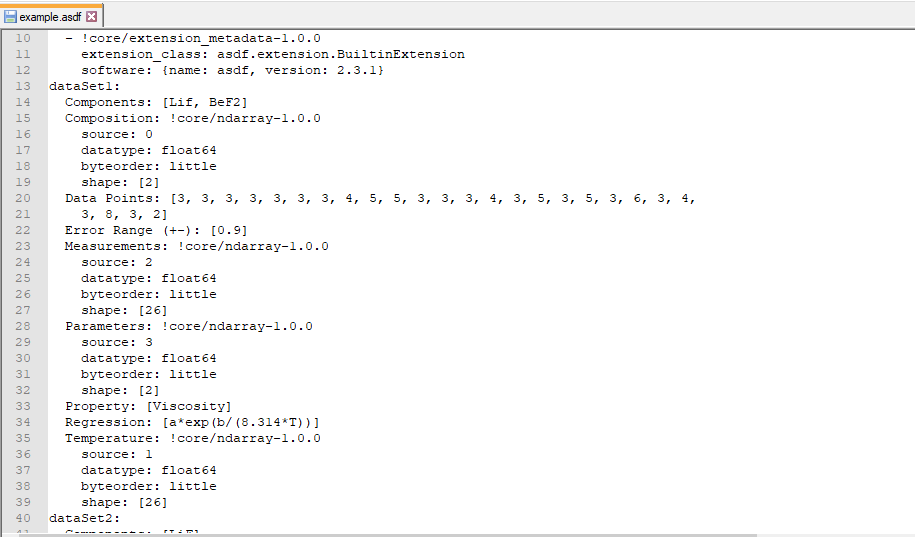
\includegraphics[width=\linewidth]{msdf/figures/asdfEx1.PNG}
\end{minipage}%
\begin{minipage}{0.5\textwidth}
  \centering
  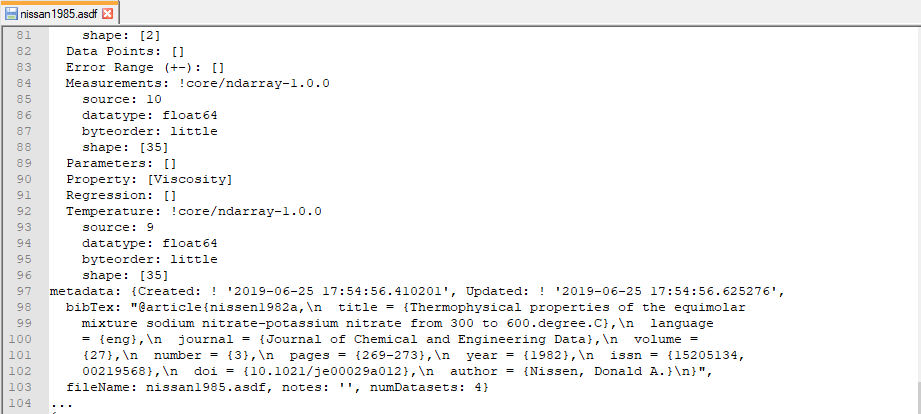
\includegraphics[width=\linewidth]{msdf/figures/asdfEx2.PNG}
\end{minipage}
\caption{Example of an asdf file structure, with a) depicting a dataset structure and b) depicting the metadata}
\label{fig:asdfExample}
\end{figure}

\subsection{Introduction to Parser}
The parser source code is contained in the file \textit{ooASDF.py} located in the \textit{Director} folder, it is written to scan excel file containing experimental data points as well as text files containing citation information and create asdf file with the proper tree structure and syntax as shown in figure \ref{fig:asdfExample}. Before using the parser, it is necessary to prepare two files, an Excel file containing the raw data and optional information in a specific structure and a text file containing reference information in a bibTeX format. An example Excel file is shown in figure \ref{fig:excelEx}. Note that each asdf file is reserved for a single source, so if a single report or book contains multiple data sets for multiple salts or properties it is necessary separate them into new identical  Excel sheets, the Parser will scan all Excel sheets and treat them all equally. It is important the data input for the excel files matches the units showcased in Table \ref{tab:unitStandards}. The information with red lettering is a requirement to fill out, but anything in green is optional and any additional information the user wants to convert can be added by going down the rows.

\begin{figure}[h]
    \centering
    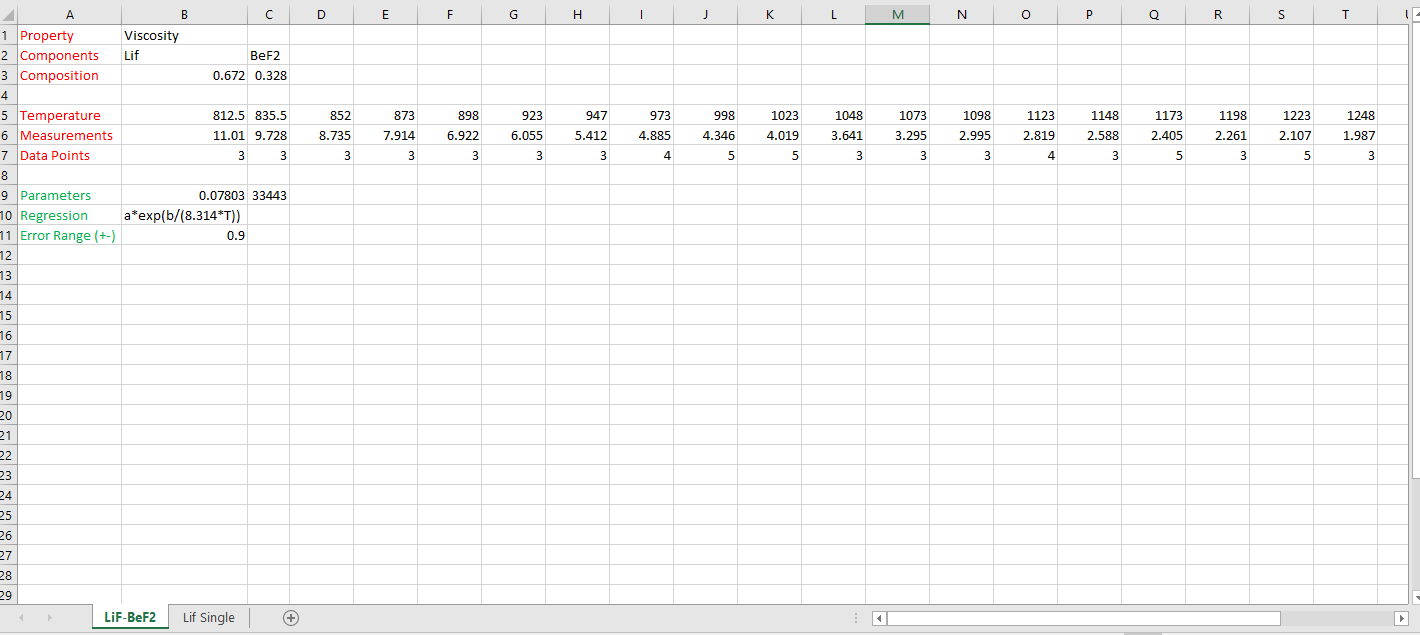
\includegraphics[width = 0.7\textwidth]{msdf/figures/excelEx.PNG}
    \caption{Example Excel file with correct structure and syntax}
    \label{fig:excelEx}
\end{figure}

\begin{table}[h]
    \centering
    \caption{List of physical properties currently in the database with expected associated unit and basis function to regress Temperature dependent data to parameters $a$,$b$ and $c$.}
    \begin{tabular}{c|c|c}
    \hline
    Property     & Unit & Fitting Function  \\ \hline
    Temperature     & \textdegree{}C  & N/A\\
    Density & $g/cm^3$ & $a+bT$\\ 
    Viscosity & $Pa \, s$ & $a*exp(b/(8.314T))$\\
    Surface Tension & $dyn/cm$ & $a+bT$\\
    Electrical Conductance & $1/(ohm\, cm)$ & $a + bT + cT^2$ \\
    Heat Capacity & $cal/(K\,mol)$ & $a + bT + cT^{-2}$ \\
    Vapor Pressure & $mmHg$ & $10^{a + b/T}$ \\
    Thermal Conductivity & $10^4* \, cal/(cm\,sec\,K)$ & $a + bT$\\
    \hline
    \end{tabular}
    \label{tab:unitStandards}
\end{table}

The reference file can simply be a Text File that contains reference information in bib format as raw text. One of the primary features of the project is the ability to track all the experimental data, meaning this is a requirement when creating new files. If the reference information is missing the program will throw an error.
 These two Input files should then be placed in the \textit{Input Files} folder as seen in figure \ref{fig:inputStruct} before running the program. Afterwards the Excel and reference text files will be stored in the \textit{Converted Files} folder\\

\begin{figure}[h]
    \centering
    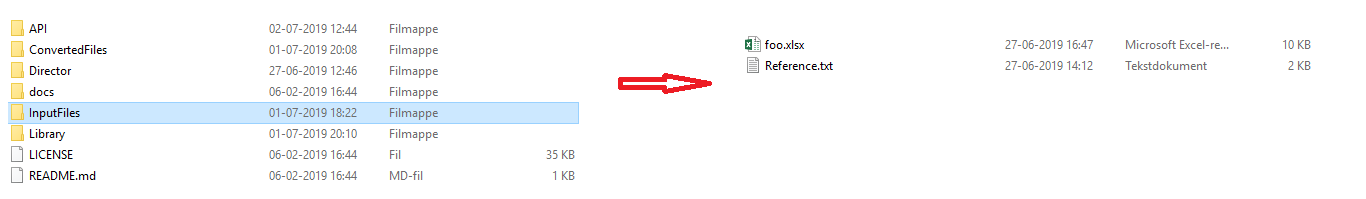
\includegraphics[width = 0.7\textwidth]{msdf/figures/input.png}
    \caption{Showcasing where to put Excel and Reference Files}
    \label{fig:inputStruct}
\end{figure}

Using the program can be done either by typing in the commands at the bottom of \textit{ooASDF.py} as shown in figure \ref{fig:ooASDFtypeLocation} file or by importing the ooASDF class from \textit{ooASDF.py}, It is important not to change the working directory when using the program and keep it the \textit{Director} folder to ensure that the manipulated files end in \textit{Library} folder. Below is a table of the functions for the program and a couple of example usages.

\begin{figure}[h]
    \centering
    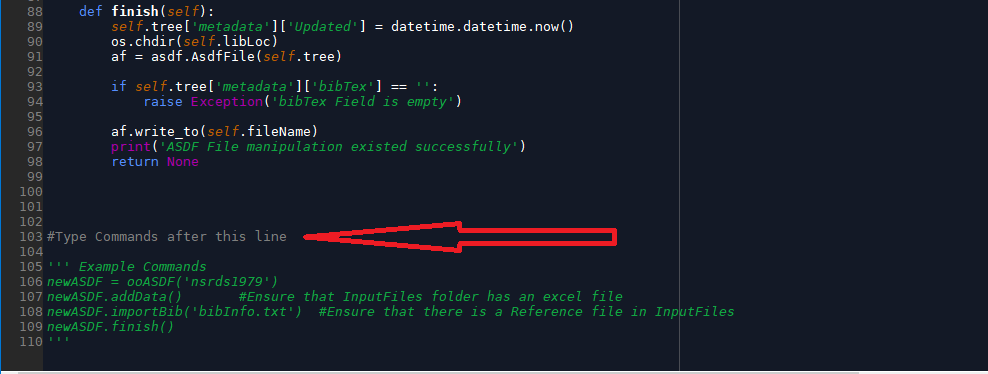
\includegraphics[width = 0.7\textwidth]{msdf/figures/ooASDFwhereToType.PNG}
    \caption{Snapshot of the program source code showcasing where to write new commands}
    \label{fig:ooASDFtypeLocation}
\end{figure}

\begin{table}[h]
    \centering
    \caption{List of ooASDF methods}
    \begin{adjustbox}{width=1\textwidth}
    \begin{tabular}{c|c}
    \hline
    Method    & Usage  \\ \hline
    ooASDF(fileName) & Constructor, opens up the specified file or creates one if it doesn't exist \\
    .addData() & Scrapes the Excel File and collects the data \\
    .importBib(fileName) & Imports the contents of fileName into a string to use as reference information \\
    .finish() & Writes the collected data into an asdf file\\
    \hline
    \end{tabular}
    \end{adjustbox}
    \label{tab:ooASDFmethods}
\end{table}


\subsubsection{Adding data to existing file}
If a file already exists in the library but data is missing and needs to be added, the reference bib file is not necessary. Filling up the Excel file akin to figure \ref{fig:excelEx} and putting it in the \textit{Input Files} should be done first. Then use the following three commands to add the data.
\begin{verbatim}
    asdfFile = ooASDF('existingFile')
    asdfFile.addData()
    asdfFile.finish()
\end{verbatim}
The first line opens up an existing datafile, the second line scans all the Excel sheets and adds the data to it and the third line updates the datafile with the scraped information and updates the metadata.

\subsubsection{Creating new file}
Creating a new datafile is very similar as updating an existing one, except now it is necessary to include the reference information along with the Excel file in \textit{Input Files}

\begin{verbatim}
    newFile = ooASDF('newFile')
    newFile.addData()
    newFile.importBib('bibInfo.txt')
    newFile.finish()
\end{verbatim}
This follows a very similar workflow as for adding data except now the first line creates the new datafile with the specified file name and the third line scans in the reference information and adds it to the metadata. Trying to build a new datafile without using .importBib() method will result in an error due to missing source.

\subsection{Introduction to API}
The API source file is \textit{api.py} located in \textit{API} folder. This part of the program handles all data extraction from the molten salt data library while also containing some data processing features such as regression, model fitting and visualization. Using the api to do dataprocessing is simply importing the \textit{api} class or use the \textit{api.py} source file similar to how to use the Parser and simply ask for a physical property and a salt mixture. Optionally it is possible to extract specific mixing ratios of the molten salt. After running the parser a new \textit{output.xlsx} file is created which contains the filtered information found in the data library as well as regression information if applicable. Table 

\begin{table}[h]
    \centering
    \caption{List of API functions and methods}
    \begin{adjustbox}{width=1\textwidth}
    \begin{tabular}{c|c}
    \hline
    Method    & Usage  \\ \hline
    API(Property,Salt List, \textit{Composition}) & Constructor to set up the object, the \textit{Composition} argument is optinal \\
    .scanLibrary() & Scans the entire library for matching salt mixture and physical property \\
    .organizeData() & Organizes the data into X and Y arrays ready for data analysis \\
    .regressData() & Regresses data of single mixtures to a basis function in table \ref{tab:unitStandards}\\
    .buildModel() & Builds a mathematical model of the data, currently Regression Kriging model \\
    .makePlot() & Visualizes the data in graphical format \\
    .printExcelReport() & Creates the \textit{output.xlsx} file with all the gathered data \\
    .initializeData() & Combines scanLibary(), organizeData() and printExcelReport() methods for pure data extraction\\
    .intializeFull() & Combination of all above function for full data analysis of given salt mixture \\
    \hline
    \end{tabular}
    \end{adjustbox}
    \label{tab:apiMethods}
\end{table}

Below are some example usages on the program to extract relevant information from the library

\subsubsection{Extracting raw viscosity data of $CaCl_2$}
Simply extracting raw data from library containing only viscosity data of $CaCl_2$ can be done in two commands
\begin{verbatim}
    CaCl2Dat = API('viscosity',['CaCl2'])
    CaCl2Dat.initializeData()
\end{verbatim}
Where first command creates the Python object and second command combines the API features of scanning, organizing and output into an excel file. This will result in an excel file depicted in

\begin{figure}[h]
\centering
\begin{minipage}{0.5\textwidth}
  \centering
  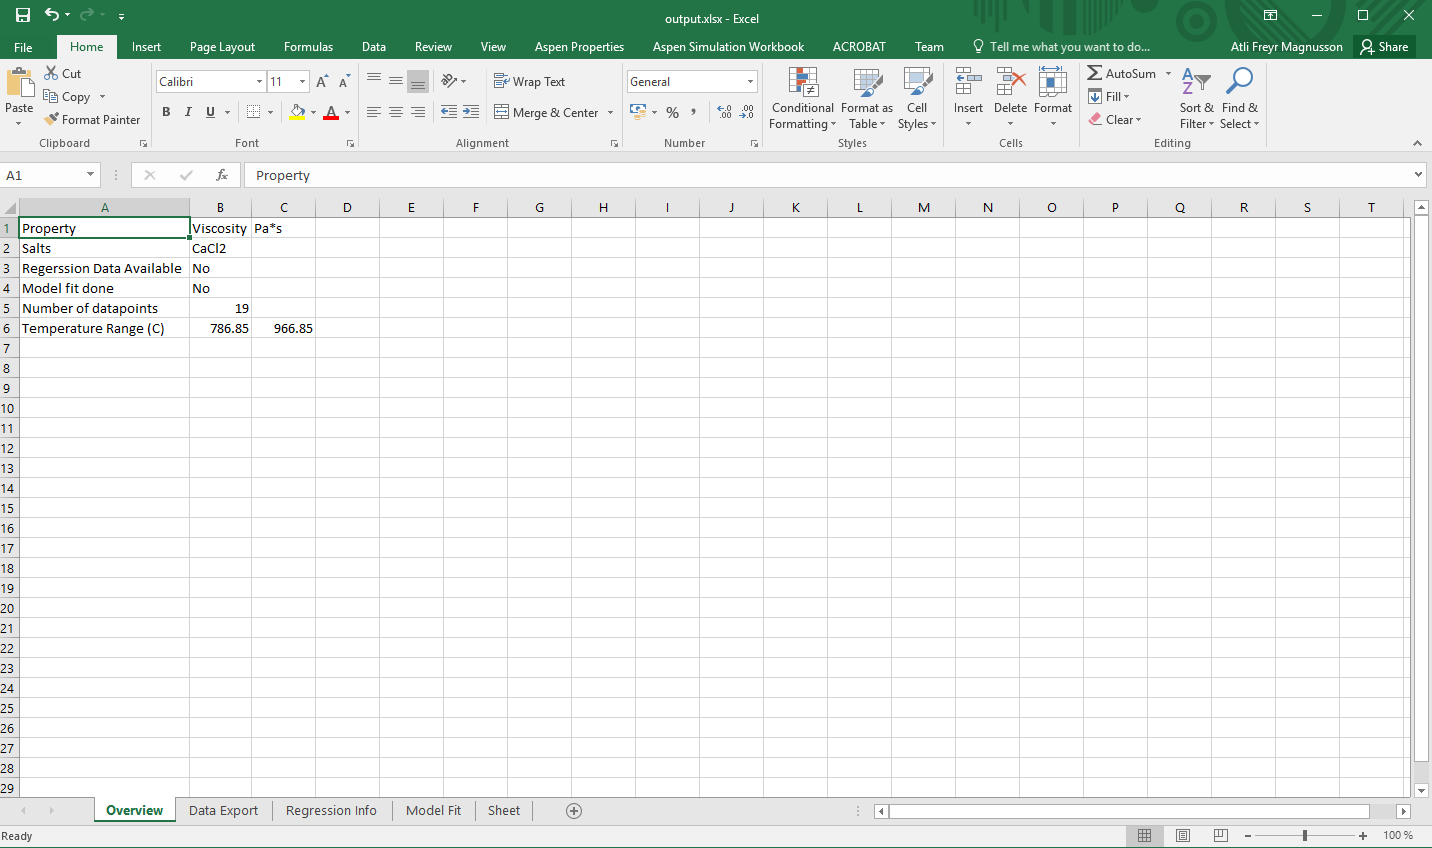
\includegraphics[width=\linewidth]{msdf/figures/caclOverview.PNG}
\end{minipage}%
\begin{minipage}{0.5\textwidth}
  \centering
  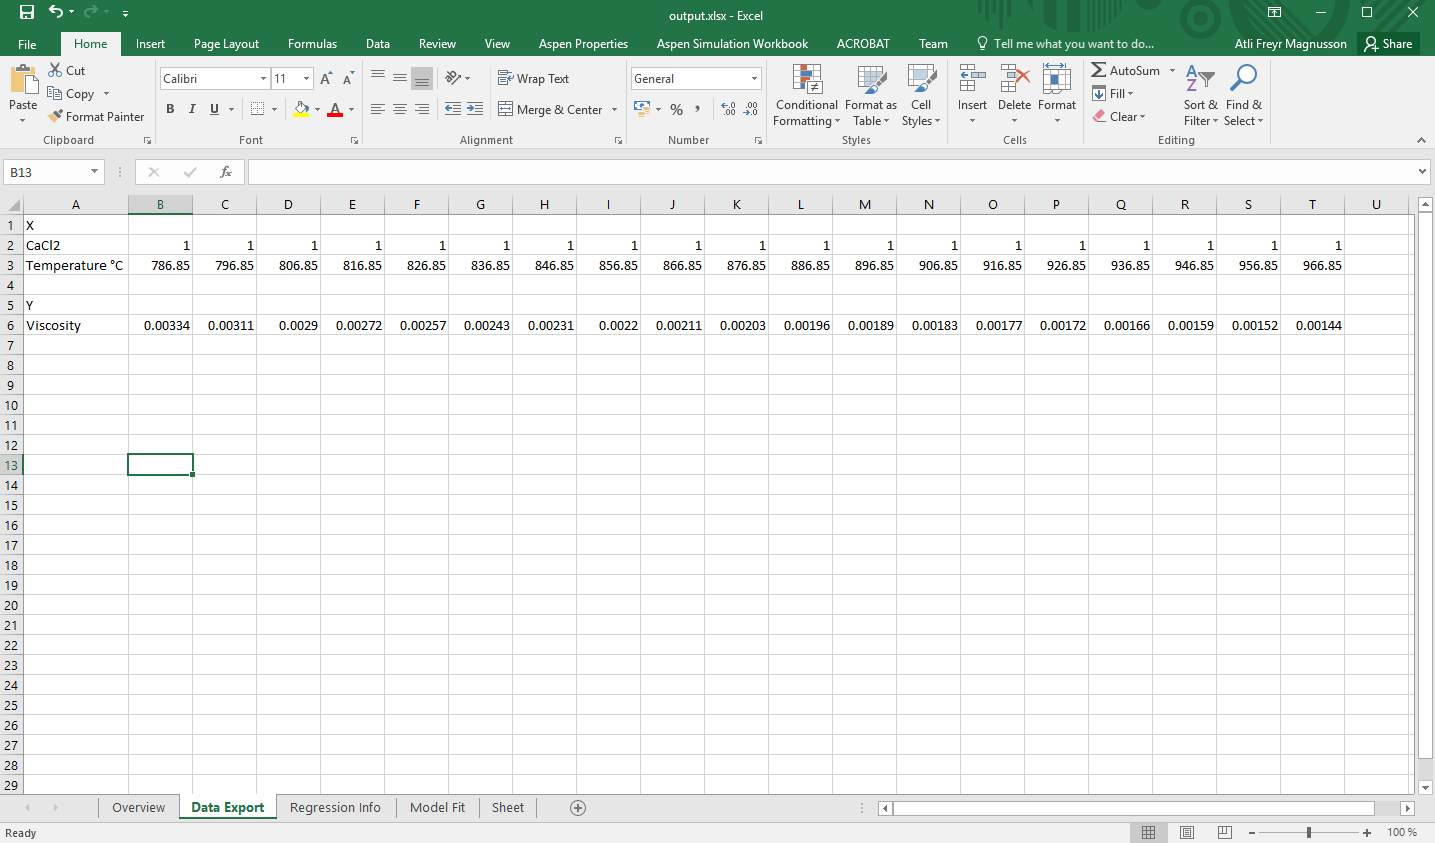
\includegraphics[width=\linewidth]{msdf/figures/caclExport.PNG}
\end{minipage}
\caption{Example Excel output when asking for viscosity data of molten $CaCl_2$.}
\label{fig:caclExcel}
\end{figure}

\subsubsection{Full regression and model building of $CaCl_2$ viscosity data}
To utilize all the data processing features implemented so far two commands are needed, similar to above commands except replace initializeData() with intializeFull().

\begin{verbatim}
    CaCl2Obj = API('viscosity',['CaCl2'])
    CaCl2Obj.initializeFull()
\end{verbatim}
This also results in the Excel information depicted in figure \ref{fig:caclExcel}, but now the Regression Info and Model Fit sheets also contain information shown in figure \ref{fig:caclFits}. The Regression Info contains the basis function used, the fitted parameters and an illustration of the regression. The Model Fit only contains an illustration of the Kriging model due to it's complexity. 


\begin{figure}[h]
\centering
\begin{minipage}{0.5\textwidth}
  \centering
  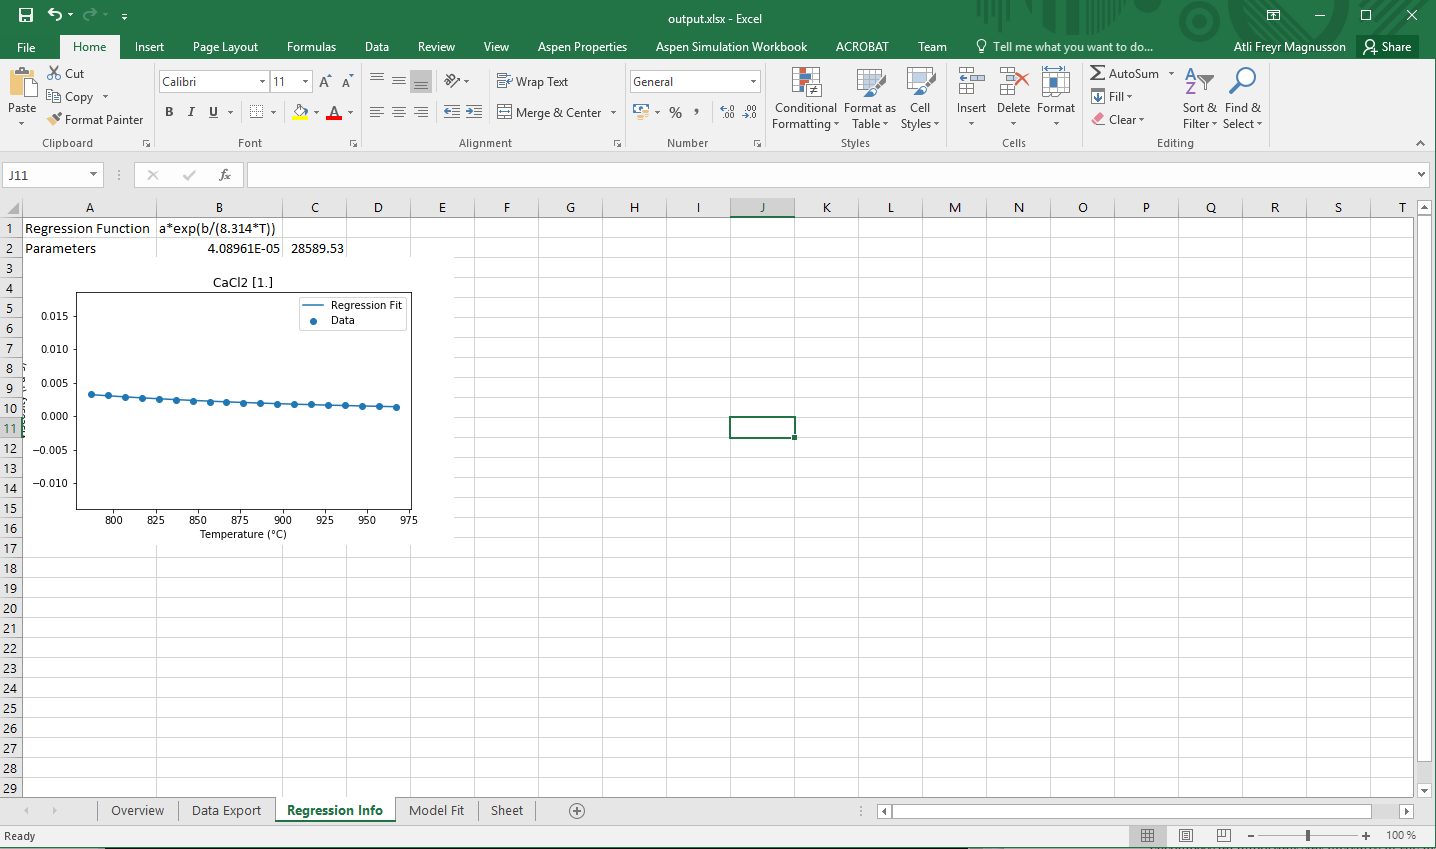
\includegraphics[width=\linewidth]{msdf/figures/caclRegression.PNG}
\end{minipage}%
\begin{minipage}{0.5\textwidth}
  \centering
  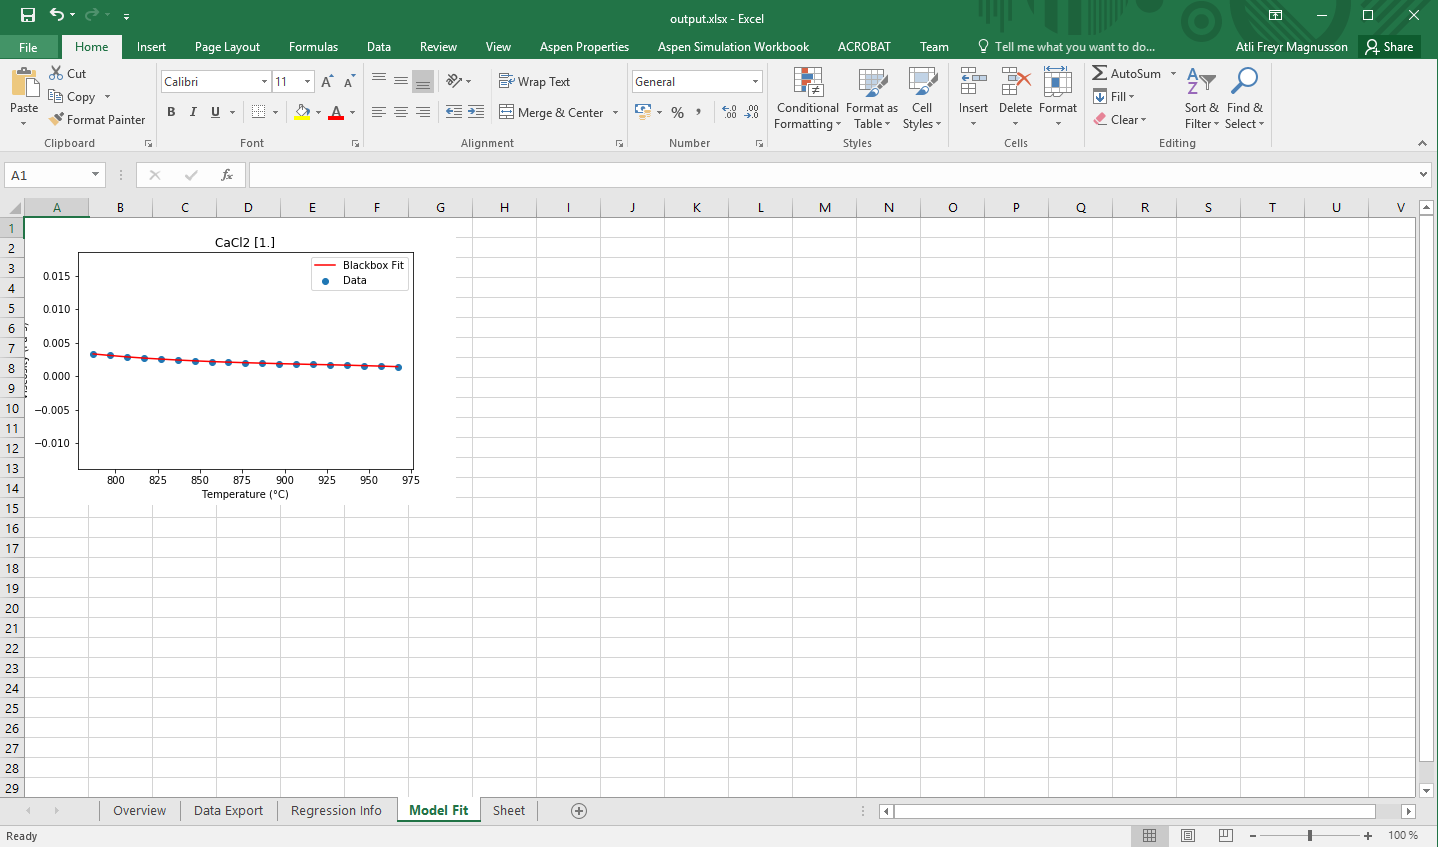
\includegraphics[width=\linewidth]{msdf/figures/caclBlackBox.PNG}
\end{minipage}
\caption{Results of Regression and Model fitting of $CaCl_2$ viscosity data}
\label{fig:caclFits}
\end{figure}


The Regression Kriging model can still be used to predict new data points. The regression model is stored in the variable \textit{fitModel} in the Python object and has the .predict() method which accepts a Temperature coordinate and outputs a prediction. A full command example:
\begin{verbatim}
    CaCl2Dat.fitModel.predict([862.52])
    >>0.002147126842301393
\end{verbatim}

\subsubsection{Analysis of a single $LiCl-KCl$ mixture with a molar ratio 20\% molar percentage of $LiCl$}
When dealing with a salt mixture that in the library holds temperature dependent data for multiple mixing ratios like for the $LiCl-KCl$ system, it is possible to specify the mixing ratio as desired with an optional mixing ratio input to the API() command.

\begin{verbatim}
    binaryMixture = API('density',['LiCl','KCl'],[20,80])
    binaryMixture.initializeFull()
\end{verbatim}
This will result in a similar \textit{output.xlsx} as for a single salt system depicted in figures \ref{fig:caclExcel} and \ref{fig:caclFits}. The \textit{fitModel} feature works under the same condition as above. Since only temperature dependence is analysed the visualization is a 2D plot exploring temperature dependence as shown in figure \ref{fig:Licl20}.

\begin{figure}[h]
\centering
\begin{minipage}{0.5\textwidth}
  \centering
  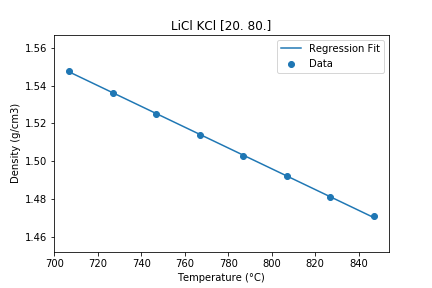
\includegraphics[width=\linewidth]{msdf/figures/LiCl20Reg.png}
\end{minipage}%
\begin{minipage}{0.5\textwidth}
  \centering
  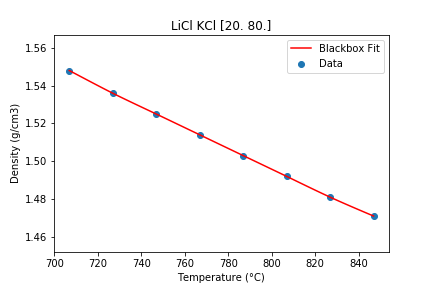
\includegraphics[width=\linewidth]{msdf/figures/LiCl20Bl.png}
\end{minipage}
\caption{Example output when asking for density analysis of 20-80 Mixture of $LiCl-KCl$}
\label{fig:Licl20}
\end{figure}

\subsubsection{Modelling density of $LiCl-KCl$ system for different mixing ratios}
Alternatively it is possible to extract the data and get a model fit for the entire system at all mixing ratios. In this case there is no regression done as now the program also analyses effect of mixing and currently we lack a basis function that accounts for both temperature and mixing dependencies. Thus only fitting done is the Regression Kriging model. To run this analysis for a salt mixture that contains data for multiple mixing ratios simply skip the mixing ratio parameter in the API() call.

\begin{verbatim}
    binaryMixture = API('density',['LiCl','KCl'])
    binaryMixture.initializeFull()
\end{verbatim}
Since this is a binary mixture we can depict the fit model as a 3D surface plot depicted in figure \ref{fig:liclsurfade}. This is done automatically for all binary mixtures, however no illustration is made for ternary or higher dimensional mixtures.

\begin{figure}[h]
    \centering
    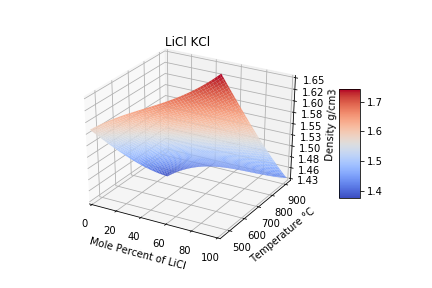
\includegraphics[width = 0.7\textwidth]{msdf/figures/LiClSurface.png}
    \caption{Surface plot of $LiCl-KCl$ Regression Kriging model predicting Density}
    \label{fig:liclsurfade}
\end{figure}

Using the fitted model is done with a similar syntax as for a single salt case but this case a mixing coordinate also has to be passed into the .predict() method. For a binary case simply put the mole percentage of the first case and then Temperature in Celsius. 

\begin{verbatim}
    binaryMixture.fitModel.predict([62.3,752.4])
    >>1.5096203630922684
\end{verbatim}
If the mixture contains more salts, then to use the prediction function it is necessary to pass the entire mixing coordinate and then supply the temperature

\begin{verbatim}
    ternaryMixture = API('viscosity',['lif','bef2','thf4'])
    ternaryMixture.initializeFull()
    ternaryMixture.fitModel.predict([0.62,0.34,0.04,895.5])
    >>0.8954644016700709
\end{verbatim}


\textit{Note}: Most salt systems currently in the library only contain a single mixture, in this case data analysis reverts to a single mixture as in 3.2.3 automatically, even if no mixing ratio was specified.\\
Example when asking for data on a $LiF-BeF_2$ mixture

\begin{verbatim}
    binaryMixture = API('density',['Lif','BeF2'])
    binaryMixture.initializeFull()
\end{verbatim}
This will results in illustrations depicted in figure \ref{fig:lifbef}.

\begin{figure}[h]
\centering
\begin{minipage}{0.5\textwidth}
  \centering
  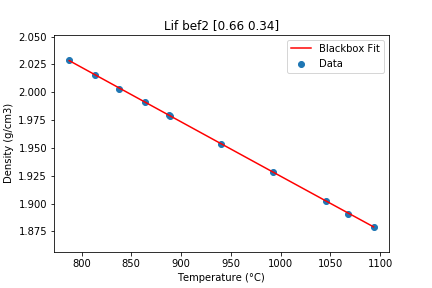
\includegraphics[width=\linewidth]{msdf/figures/lifbefRe.png}
\end{minipage}%
\begin{minipage}{0.5\textwidth}
  \centering
  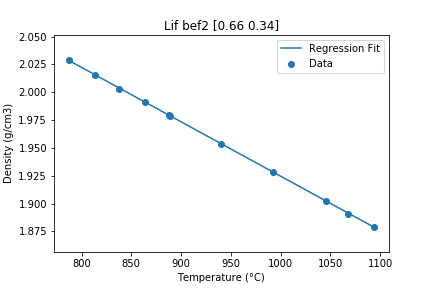
\includegraphics[width=\linewidth]{msdf/figures/lifbefBl.png}
\end{minipage}
\caption{Example output when asking for density analysis of $LiF-BeF_2$}
\label{fig:lifbef}
\end{figure}
\newpage
\section{Conclusions and future work}
In this project we started building the infrastructure for a molten salt data library. We have created a base standard for the data format and provided some tools to easily convert experimental results into the specified format as well as an easy to use tool for simple data analysis. This is however only the beginning and a lot of work is still needed before this project can be used in large scale projects in the likes of reactor design. For future work on the project we suggest to address the following issues:

\begin{enumerate}
    \item \textbf{Expand the data library} \\
    Over 100 experimental results have been converted to the proper data format and are ready to be analyzed by the tools, this only scratches the surface on how much data exists in literature. To represent a full fledged data library this needs to be expanded to encompass all important salt mixtures in the literature which could mean over a thousand sets. However the parser constructed for the project can easily add the data to the library thus expanding the data library is all about continuing the search through the scientific literature this project started.Obtaining the data from ORNL should be focused upon, as experimental data is very valuable. Another feature could be inclusion of Class-II and Class-III papers, when we have a robust Class-I data set available. The data library syntax will have to be updated on that. 
    \item \textbf{Eliminate dependencies} \\
    The Parser only accepts Microsoft Excel files for the input and the API only prints the output information in a Microsoft Excel format. This was done for convenience when starting the data collection and processing. As this project grows in scope however it's important that other alternatives are presented. This is to follow the design philosophy that the data library is accessible by everyone on multiple platforms.
    \item \textbf{Improve the mathematical modelling}
    Currently the program only supports one mathematical model when it comes to predicting physical properties of new salt mixtures which is the Regression Kriging model. This model is currently used while the dataset is still small and sparse but it will run into computational issues for larger data sets and is a blind blackbox model. The library of mathematical models to choose from should be expanded to allow for greater degree of data analysis. This could range from having alternative surrogate models such as Support Vector Regression or building a mechanistic model more grounded in the science of molten salts.
    \item \textbf{Improve user friendliness}\\
    Using the data library or any of the tools requires some basic knowledge of Python programming. However many of the fields experts may not be familiar with it or have time to learn the language. To make the library more accessible it may be necessary to develop a Graphical User Interface for the data library that retains all the features already implemented.
    
\end{enumerate}
Of course while tackling the aforementioned issues, all bugs reported should be fixed as soon as possible and code should be readily maintained to ensure that the project remains in a usable state for the foreseeable future.


% -------------------------------------------------------------------
% Bibliography
% -------------------------------------------------------------------

\bibliographystyle{abbrv} 
\bibliography{mybibliography} 


% -------------------------------------------------------------------
% Appendices
% -------------------------------------------------------------------
 \newpage
\begin{appendices}
\section*{Appendix A}
\setcounter{table}{0}
\renewcommand{\thetable}{A\arabic{table}}

\begin{table}[h]
    \centering
    \caption{List of salts and salt mixtures currently in the datasets as well as the total number of experimental data}
    \begin{tabular}{c|c}
    Salt Mixture     & Number of Datasets  \\ \hline
    $BeF_2$     & 1 \\
    $NaNO_3-KNO_3$ & 4 \\
    $KNO_3$ & 7 \\
    $MgCl_2$ & 6 \\
    $CaCl_2$ & 7 \\
    $LiCl-KCl$ & 37 \\
    $AlCl_3$ & 1 \\
    $LiF$ & 4 \\
    $Li_2CO_3$ & 6 \\
    $Na_2CO_3$ & 6 \\
    $K_2CO_3$ & 5 \\
    $LiNO_3$ & 5 \\
    $NaNO_3$ & 6 \\
    $Li_2SO_4$ & 4 \\
    $Na_2SO_4$ & 9 \\
    $K_2SO_4$ & 1 \\
    $LiBr$ & 5 \\
    $LiI$ & 5 \\
    $LiF-BeF_2-ThF_4$ & 5 \\
    $LiF-BeF_2$ & 1 \\
    $LiF-BeF_2-ZrF_4$ & 1 \\
    $LiF-BeF_2-ZrF_4-UF_4$ & 1 \\
    $NaBF_4-NaF$ & 2 \\
    $KNO_3-NaNO_2-NaNO_3$ & 3 \\
    $NaNO_2$ & 1 \\
    \hline
     Total & \textbf{133} \\
    \end{tabular}
    \label{tab:listofSalts}
\end{table}

\end{appendices}

\end{document}
